%----------------------------------------------------------------------------
\chapter{Az elvégzett munka}
%----------------------------------------------------------------------------

Ebben a fejezetben a megvalósított alkalmazás tervezését és megvalósítását részletezem, helyenként indokolva a hozott döntéseket.

%----------------------------------------------------------------------------
\section{Rendszerterv}
%----------------------------------------------------------------------------

A rendszerterv a célkitűzéssel kezdődik, majd a kollaborációs követelmények tisztázásával és a rendszer felépítésével folytatódik.

\subsection{Célkitűzés}

A szakdolgozatom célkitűzése egy olyan alkalmazás, ami vizuális programozási nyelvek vagy adatmodellezési nyelvek fejlesztését teszi lehetővé kollaboratívan és mindezt egy böngészőalkalmazás keretein belül.

A másodlagos cél egy teljes alkalmazás építése Javascript alapon korszerű technológiák felhasználásával mint AngularJS, NodeJS, MongoDB.

A Lucidcharts és hasonló webalkalmazásokból ihletődve egy annál minimalistább felület a cél, a Lucidcharts modellező alkalmazás minél tágabb modellezési nyelv halmazt próbál lefedni, de nem támogat kódgenerálást és nem lehet kinyerni a gráf reprezentációját valamilyen szöveges formátumban. Igaz, a Lucidcharts gráfja is HTML elemekből áll, és nem lenne lehetetlen egy diagram DOM részfáját transzformálni valamilyen használható formára és az alapján kódot generálni, de egy kézenfekvő próbléma ezzel az, hogy egy komoly függőség alakul ki egy más által fejlesztett szoftverre.

Mivel ez egy webalkalmazás, bármikor megváltozhat ez a grafikus interfész és újra kell írni a transzformációt. 

A Jsfiddle webalkalmazás is ihletet jelentett, mivel egy elég hasznos fejlesztői eszköz akár webalkalmazás részletek prototipizálására kollaboratívan. Lucidcharts-szal szemben csupán egy HTML, CSS és Javascript fejlesztőkörnyezet, viszont egy weboldalt lehet a kód alapján létrehozni a böngészőben. 


A koncepció nagyjából a két alkalmazás közötti átmenet, kiegészítve azzal, hogy a gráf alapján kódot lehessen generálni és azt a kódot fel lehessen használni egy külső alkalmazásban. Ebben a formában használható lenne mint tanítási eszköz, a vizuális eszközkészlet kibővítésével testreszabható vizuális programozási nyelveket lehet létrehozni.

A felhasználás amire én terveztem az domén-specifikus modellezéssel való kiegészítése tetszőleges alkalmazásnak. Két példával is ábrázolom ezt az ötletet:
\begin{enumerate}
\item Egy interaktív videó webalkalmazás\footnote{vidzor.com} egyik fő funkciója a ``video linking'', amivel a videó lejátszás közben felhasználói eseménytől függően dinamikusan egy másik videó játszódik le -- hasonlóan a weboldalak esetében használt linkre. De ennél még érdekesebb az, hogy több ágon is lehet továbbhaladni egy videonézés közben, más szóval interaktív a video nézési élmény. 

Ekkor eléggé triviális azt gondolni, hogy ez egy gráf lehet reprezentálni, ahol a videók csúcsok és a kimenő élek az elágazási lehetőségek. Nagyobb gráf esetén átláthatatlanná válhat egy ilyen videó élmény szerkesztője; én egy ilyen funkciónak a támogatására képzelem, hogy alkalmas a szakdolgozatom munkája. Megjegyzem, hogy ehhez ki kellene terjeszteni a szerkesztőt a video galéria letöltésére többek között. 
\item Egy munkafolyamat menedzselő alkalmazás: bizonyos állapotátmenetekkel modellezhető folyamat alapján állítanak elő termékeket. A webalkalmazás ami ezt a folyamatot kiegészíti állapotfüggő webes felülettel kiegészíthető egy olyan komponenssel ami nem csak, hogy vizualizálja az állapotgépet, de szerkeszthetővé teszi és kódot is fordít, ami beépül mint állandó komponens. 

\end{enumerate}

A szakdolgozat keretein belül én a második felhasználói esetet mutatom be példaként: a szerkeszthető állapot diagram alapján egy állapotgép osztályt fordítok le, majd ezt betöltöm egy külső alkalmazásba, példányosítom és használom.

\begin{figure}[!ht]
\centering
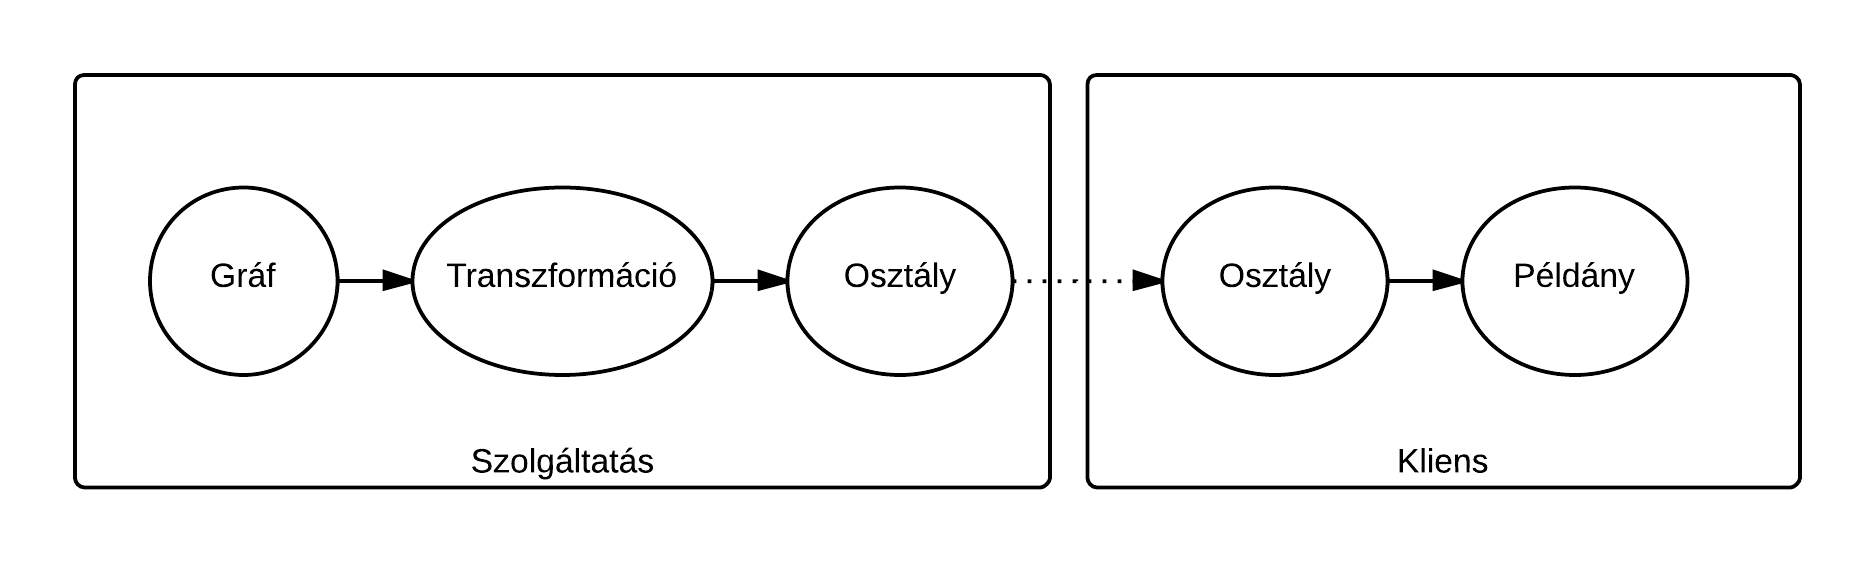
\includegraphics[width=\textwidth,height=\textheight,keepaspectratio]{figures/flow.png}\\
\caption{A szolgáltatás nagy vonalakban}
\label{fig:flow}
\end{figure}

A ~\ref{fig:flow} ábrán felhasználói szemszögből nézzük az alkalmazást, ezt el lehet érni akár szolgáltatásként a weben, vagy a kész munkára építve belső hálózaton saját magunk üzemeltethetünk egy példányt. A felhasználó a felületen létre tudja hozni a diagramot és a felületen létre tudja hozni a transzformációs logikát, a szerver majd értelmezi a kettőt és lefordítja kóddá, ami példáúl egy Javascript osztály lesz. A felhasználó majd ezt a komponenst a saját alkalmazásában szeretné használni és a szolgáltatás megfelelő API végpontján eléri ezt a kódot és a saját alkalmazásában példányosítja.





\subsection{Kollaboráció}

Mivel kollaboratív alkalmazásról van szó elsőbbségi szempont az ellentmondó, nagyjából egyidejű változtatások konfliktusait feloldani. Felmerült ötletként a Google Docs-ban alkalmazott Operational Transformation megoldás amiben folyó szöveg egyidejű módosítása van megoldva ``előbb-útóbbi'' konzisztencia elérésével. Az Operational Transformation algoritmust nem triviális implementálni, viszont vannak nyílt forráskódú megoldások rá\footnote{http://www.sharejs.com}. Nem ezen a vonalon indultam el, mert nehézkesnek gondoltam annak a rétegnek a fejlesztését ami a DOM-ban levő gráfot szöveggé- és vissza transzformálja akkor is, ha meg van oldva a különböző kliensek által látott szövegreprezentáció kollaboratív változtatása. 

Erre az alternatíva ami végül kiválasztásra került egy meglehetősen pehelysúlyú megoldás: a gráf módosítását jól meghatározott eseményekként defineálom és ezek az események a többi felhasználóhoz Websocket broadcast üzeneteken keresztül jutnának el. Egy példa esemény egy entitás módosítása: az egyik kliens böngészőjében elhúzunk egy elemet, a kliensoldali kód a szervernek egy kérésben szól a módosításról, a szerver perzisztálja az adatot és Websockets broadcast üzeneten keresztül értesíti a többi résztvevőt. Ilyenkor az esemény üzenet a módosult adatot is tartalmazza. 

Ebben a megoldásban igazából semmi konfliktus feloldás nincsen és a továbbiakban be fogom mutatni, hogy ez nem is feltétlenül szükséges. Először is nézzük meg, hogy milyen jellegű konfliktusokról lehet szó; a közösen manipulált elemeket lehet egyidejűleg létrehozni, törölni és módosítani -- feltételezve két szereplőt -- a következő esetek relevánsak:

\begin{enumerate}
\item { \emph{törlés - törlés}}: Ha majdnem egyszerre ketten törlik ugyanazt az entitást, akkor csak kezelni kell kliens és szerver oldalon, hogy a később érkező törlés művelet ne okozzon hibát. 
\item { \emph{módosítás - módosítás}}: Itt két eset lehetséges:
\begin{enumerate}
\item Különböző attribútumok változnak. Ekkor, ha csak a változásokat küldjük el, akkor triviálisan összefésülhetők a különböző attribútumokra vonatkozó egyidejű változások, ha nem, akkor igazából a következő esetről beszélünk,
\item Ugyanazok az attribútumok változnak. Ekkor sajnos arról beszélünk, hogy, példáúl, egyidejűleg az első felhasználó jobbra 
húzta, a másik felhasználó balra húzta az objektumot és a később történt esemény fog végül érvényesülni. 

Az első kérdés ami felmerül itt az, hogy ez egyáltalán próbléma-e? Próbléma, mert ugyan a mozgatás elvesztése apró művelet és könnyen megismételhető, de, ha egy hosszú szöveg beírásáról van szó egy attribútum mezőbe, akkor nem kívánatos elveszíteni azt, ha a másik résztvevő kitörli a régi változatot. Egyszerű modellek szerkesztésénél mint egy állapot diagramnál a hosszú szövegek beírása nem tipikus próbléma. 

Jó esetben körülbelül 100 ms alatt mindenkihez eljutnak az események, ez azt jelentené, hogy nem lehet annyira gyakori ez a próbléma, hogy egy verziókezelő rendszerhez hasonló megoldással lassítsuk a felhasználók munkafolyamatát.

Egy egyszerű felhasználói élmény javítás egy jelzés lesz, ami úgy néz ki, hogy minden felhasználó látja, hogy ki éppen milyen objektumot jelölt ki színekkel jelölve. Ha valaki más ki szeretné törölni az objektumot aminek a hosszú tartalmát éppen írjuk, akkor a rendszer legalább mutatja, hogy azt valaki kijelölte. Ez a megoldás egyik fő előnye, hogy nem bonyolítja egyáltalán a munkafolyamatot példáúl a zároláshoz képest.

\end{enumerate}
\item { \emph{módosítás - törlés }} Ez a szituáció ugyanaz mint az előző. A fent említett megjelölés egy megoldás, de egy visszavonás művelet megnövekedett komplexitás árán megoldaná teljesen a próblémát.
\end{enumerate}

A létrehozás-törlés, létrehozás-módosítás és létrehozás-létrehozás kombinációk nem fordulhatnak elő ugyanazon az entitáson, hiszen nem lehet olyat módosítani egyidőben amit a másik kliens éppen létrehoz.

Ha a két művelet két különböző csúcsot érint, akkor nincs próbléma, mert triviálisan mindkét művelet érvényesül, ha a egy csúcsot és egy hozzá tartozó élet érint, akkor sincs gond, mert a csúcs törlése maga után vonja az él törlését is. 

\subsubsection{Zárolás}

Szigorú zárolás alatt az értendő, hogy valamilyen algoritmus lehetővé teszi, hogy a felhasználó módosítások elől védje a diagram bizonyos részét és itt a módosítások nem kívánt elveszítéséről van szó általános egyidejű szerkesztés közben. Elképzelhető, hogy van értelme ``véglegesíteni'' egy diagramot és akkor megtilthatjuk zárolással a további módosításokat. Elég könnyű találni próblémákat a részleges zárolás ötletében, talán a legkézenfekvőbb a deadlock kialakulása: ketten egyszerre akarnak egy olyan halmazt módosítani, amit nem lehet egyszerre zárolni és egymást kizárják. Tehát nő a komplexitás azzal, hogy a rendszernek ezt meg kell akadályoznia és azt is meg kell akadályoznia, hogy túl sokáig ne maradon érvényes a zár.  

Az előnye a pehelysúlyú kollaborációs megoldásnak az egyszerűség és a remélhetőleg jobb felhasználói élmény ami abból eredhet, hogy visszaigazolás nélkül módosul a felhasználó felületén a diagram a saját beavatkozása után. Egy olyan alkalmazásnál ami egy nem-kollaboratív offline alkalmazással versenyzik létfontosságú a kis reakcióidő a felületen. Az egyszerűség maga után vonja a könnyebb karbantarthatóságot és kisebb hibalehetőséget.   

A hátránya az, hogy nem garantálja, hogy mindenkinek érvényesülnek vagy megmaradnak a módosításai.

\subsubsection{Eltérések detektálása}

Egy funkció ami jelzi, hogy két felhasználó eltérő diagramot lát holott ugyanazt kellene, hogy lássák -- nevezzük eltérés detektálásnak -- két szempontból is hasznos lesz: egyrészt a teljesítményelemzés során fel lehet használni arra, hogy a kollaborációs megoldás hatékonyságát vizsgáljam különböző paraméterek mellett, másrészt felhasználói élmény szempontjából szükséges, hiszen, ha eltérést vesz észre az algoritmus, akkor a diagram újratöltésével orvosolható a próbléma. 
A kérdés az, hogy mi az amit összehasonlítunk ilyenkor? A teljesítményt és a sávszélességet szem előtt tartva egy egyszerű megoldás egy hash értéket számolni a diagramból majd ezt összevetni a többi kliens által kiszámolt értékkel.

Felmerült a kérdés, hogy a diagram hash logika hol legyen: kliensoldal, szerveroldal vagy mindkettő. Kezdjük ott, hogy a kliensoldalon mindenképpen van rá szükség, viszont a szerveroldalon a hash kiszámolásához mindig kell az egész diagram a memóriában, ez sok queryt jelenthet, másrészt a kliensoldalon úgyis mindig be van töltve az egész diagram. Ha kihagyom a szerver oldalt belőle, akkor Websocket alapú megoldás eléggé kézenfekvőnek tűnik a több kliens összeegyeztetése szempontjából.

Másik kérdés, hogy, hogyan oldható meg az, hogy ugyanabban az időben normális körülmények között előfordulhat, hogy ketten nem ugyanazt a dokumentumot látják átmenetileg. Erről bővebben a ~\ref{subsec:hashref} fejezetben lesz szó.



\subsection{A rendszer felépítése}

\begin{figure}[!ht]
\centering
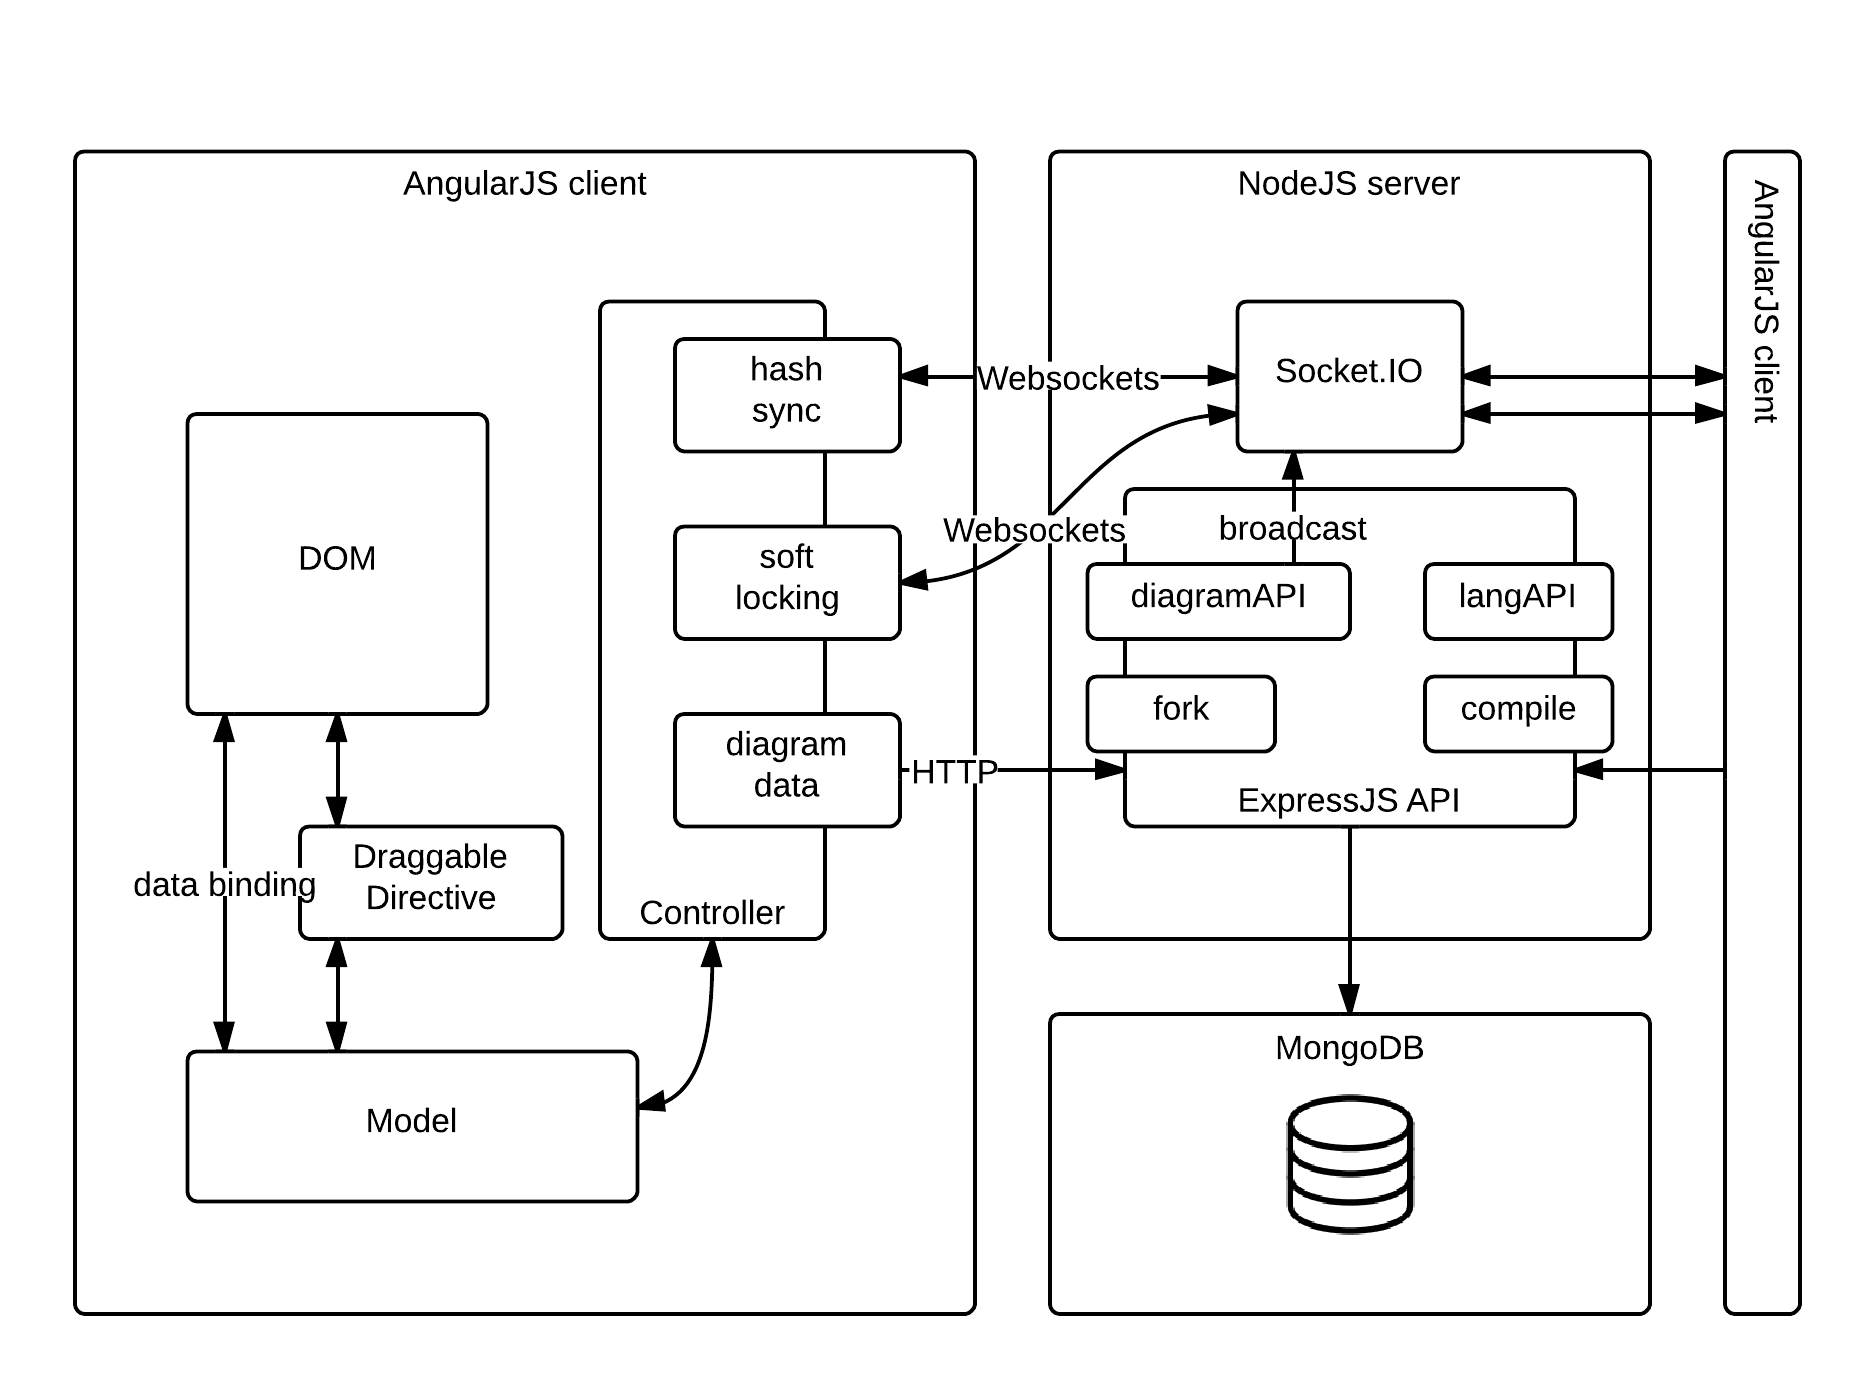
\includegraphics[width=\textwidth,height=\textheight,keepaspectratio]{figures/Rendszerterv.png}\\
\caption{A rendszer architektúrája}
\label{fig:arch}
\end{figure}

\subsubsection{Kliens oldalon}

A kliens oldal egy AngularJS alkalmazás ami Model-View-Controller paradigmára épül.  


\begin{itemize}
\item Adatkötés segítségével a modellben tárolt diagram frissen tartja a DOM-ban levő HTML elemekből álló diagramot, 
\item a manipulálható diagram entitás, a legbonyolultabb vizuális elem, egy direktíva komponenssel van megvalósítva elszigetelve azt a logikát amivel kirajzolja magát. Ez a direktíva a modell rétegen keresztül kommunikálhat a kontrollerrel és a keretrendszer gondoskodik a DOM-ba helyezésért,
\item a kliensoldali modell réteg nem más mint a \$scope kontextusában deklarált objektumok, ezt a kontrollerben meghatározott socket üzenet kezelők és API hívások módosítják. Adatkötés során bizonyos felhasználói események is közvetlenül a modellt változtatják,
\item a kontroller AngularJS-ben egy egyszerű függvény, amibe a keretrendszer függőségeket injektál, a legfontosabb ezekből a \$scope, ami összeköti a modell és a kontroller réteget. A kontrollerben deklarált \$scope-hoz kötött üzleti logika a DOM-ban is elérhető. A főbb funkciók amik a kliens oldalon vannak megvalósítva:
    \begin{itemize} 
    \item a közösen szerkesztett diagram frissítése és mentése: a felhasználó okozta módosítások egy szerveroldali API segítségével perzisztálódnak, mások által módosított adatok websocket üzeneteken keresztül érkeznek, 
    \item a ``soft locking'' nyilvántartja websocket üzenetek alapján, hogy ki szerkeszti éppen a diagramot és diagram elemek kiválasztásakor a többi résztvevőt értesíti. A többi résztvevőnek a diagramjában a felhasználóhoz rendelt színnel jelezve van, hogy melyik entitást jelölte ki,
    \item a ``hash sync'' a diagram módosulásakor lenyomatot számol a diagram elemeiből és Websocket üzeneteken keresztül értesíti a többi klienst, ha tartósan olyan lenyomatot küldenek, ami nem szerepelt a helyi legútóbbi lenyomatok közt, akkor kijelenthetjük, hogy eltér a két diagram valami hiba miatt. 
    \end{itemize}
\end{itemize}

\subsubsection{Szerver oldalon}

A szerver oldal egy NodeJS alkalmazás MongoDB adatbázissal.   

\begin{itemize}
\item A diagram módosításához számos API végpont van, ezek ExpressJS segítségével vannak implementálva, a MongoDB adatbázisba mentenek és egyes hívásoknál a SocketAdapter-en keresztül broadcast üzeneteket küldenek a csatlakozott kliensekhez,
\item a SocketAdapter egy általam fejlesztett csomagoló a Socket.IO keretrendszer köré ami beállítja a munkamenethez szükséges websocket üzenetkezelőket és menedzseli a felhasználók -- megnyitott diagram alapján -- a megfelelő socket szobába rendelését. A kliensek a szerveroldali socket szervert használják egymással való Websocket kommunikációhoz, 
\item a ``language API'' az a lefordított diagramokat teszi elérhetővé publikus API-n keresztül, ezt példáúl a NodeJS Repl\footnote{Read, Eval, Print, Loop - egy javascript parancssor NodeJS-hez} be tudja tölteni,
\item a ``compile'' modul az adatbázisból kinyeri a diagramot és a transzformációs template-t és lefordítja, így jön létre példáúl egy Javascript osztály a diagram alapján, ennek a kódját adatbázisba menti, 
\item a ``fork'' funkció létrehoz egy új diagramot egy másik alapján, ez azért van szerveroldalon, mert egy bonyolultabb adat ``deep-copy''-jára van szükség, és mivel MongoDB nem támogat relációkat, óvatosan kell implementálni az új elemek létrehozását.
\end{itemize}

%----------------------------------------------------------------------------
\section{Adatbázis}
%----------------------------------------------------------------------------

A kliens oldalról nézve egy felhasználói diagram fő elemei az entitások és a köztük lévő kapcsolatok (vagy csúcsok és élek a gráfban). 


\begin{lstlisting}[label=entity,caption=Egy gráf csúcs -- vagy entitás -- reprezentálása az adatbázisban]
{
    "_id" : ObjectId("52486e8e9b7f14a725000001"),
    "position" : {
        "top" : 312.9618225097656,
        "left" : 607.920166015625
    },
    "title" : "Alszik",
    "document" : "5242aa48ddda9b0000000001"
}
\end{lstlisting}

Az \lstinline{entities} kollekcióban tárolva vannak a diagram entitásai. Lehetne egy kollekcióban tárolni mindent ami egy diagramhoz tartozik, de azért kézenfekvő külön kollekcióban tárolni az entitásokat, mert az egyedi azonosítójukra szükség van a kliens oldalon is. A legegyszerűbb az egyedi azonosítót az adatbázisra bízni és a létrehozás API hívás válaszában meg is érkezik az azonosító és adatkötés segítségével egyből a DOM is frissül.  

A \lstinline{position} attribútum konkrétan a kliensoldali CSS pozícionálásra van használva, a document attribútum egy idegen kulcs lenne, ha relációs adatbázisról beszélnénk, de valóban annak a dokumentumnak az azonosítóját tárolja aminek része.

\begin{lstlisting}[caption=Egy diagram és élei reprezentálása az adatbázisban]
{
    "_id": "524b08b1b7f4db8e68000001",
    "connections": [
    {
        "from": "524b08b4b7f4db8e68000002",
        "to": "524b08bdb7f4db8e68000003",
        "label": "valami"
    },
    ...],

    "author": "alma",
    "title": "Egy diagram" 
}
\end{lstlisting}

Az élek nicsenek külön kollekcióban, hanem csak egy tömbben találhatóak a diagram rekordban. A \lstinline{from} és \lstinline{to} attribútumok a ~\ref{entity} ábra rekordjaira utalnak. Mivel nincsen idegen kulcs fogalma MongoDB-ben, ez a reláció nincs ellenőrizve constraint-ek segítségével, ez azt jelenti, hogy, ha megváltozik egy entitás azonosítója, akkor nem változik meg a \lstinline{connections} tömb tartalma és ez adatbázis sem jelez hibát. Ha mégis megtörténne ilyen, a kliensoldalon a beazonosítatlan él végpontok élei kitörlődnek a diagramból. 

Nem biztos, hogy ez optimális felosztás és annak is lennének előnyei, hogy minden ami a dokumentumhoz tartozik egy kollekcióban van és gyakorlatilag egy dokumentum lekérdezéséhez csak egy rekordot szükséges adatbázisból lekérni. Egyrészt implementálni kell egy azonosító generálás mechanizmust ami az adatbázistól független, viszont nagyon leegyszerűsítené a diagram másolást.

A diagram másolás a jelen séma mellett megköveteli azt, hogy az összes idegen kulcsot kicseréljem az új entitás rekordokban és az új él tömbben.



%----------------------------------------------------------------------------
\section{A szerver oldali alkalmazás}
%----------------------------------------------------------------------------

A fontosabb főleg szerveroldalon megvalósult funkciók következnek.

%----------------------------------------------------------------------------
\subsection{API}
%----------------------------------------------------------------------------

Az AngularJS kliens egy API-n keresztül kommunikál a szerverrel a dinamikus tartalom lekérdezése és mentése céljából. Ez az API JSON adatokat szolgáltat, amit akár módosítás nélkül fel lehet használni a kliens oldalon betöltve egy AngularJS modellbe; ugyanígy az API-nak beküldött új JSON objektumok módosítás nélkül a MongoDB adatbázisba íródnak. Az API több csomagoló függvényből áll, minden entitás típusra egy; egy ilyen csomagolófüggvényben a létrehozás, törlés, módosítás és olvasáshoz implementáltam függvényeket és ezeket a függvényeket require segítségével betöltöm a \lstinline{routes} modul \lstinline{index.js} fájlba, ahol példányosítom. Két függősége is van egy ilyen API modulnak: az adatbázis kapcsolat és a socket szerver példány referenciája.

\begin{lstlisting}[caption=API végpontok bekötése az alkalmazás URL szabályai közé]
    var DocumentApi = require('./api/docs.js');
    module.exports = exports = function(app, db) {
        sa = new SocketAdapter(app);
        api = new DocumentApi(db, sa);
        app.get('/api/docs', api.docs);
        app.get('/api/docs/:id', api.doc);
        app.post('/api/docs', api.adddoc);
        app.put('/api/docs/:id', api.updatedoc);
        app.delete('/api/docs/:id', api.deletedoc);
    ...
    }

\end{lstlisting}

\begin{lstlisting}[caption=Diagram API és annak egy metódusa]
module.exports = function (db, sa) {
  var docs = db.collection("docs");

  this.deletedoc = function(req, res) {
    var oid = mongo.BSONPure.ObjectID(req.params.id)
    docs.remove({_id: oid}, function(err, removed){
      res.json(removed);
    })  
  ...

\end{lstlisting}

Amikor id-ra hivatkozunk mindig szükséges egy \lstinline{BSONPure.ObjectID} példányba csomagolni az azonosítót, mert csak úgy lehet felhasználni MongoDB lekérdezésben.

%----------------------------------------------------------------------------
\subsection{Kétirányú kommunikáció}
%----------------------------------------------------------------------------

Ha azt nézzük, hogy egyidejűleg \emph{x} darab diagramot szerkeszt diagramonként \emph{y} darab különböző felhasználó, akkor felmerül az a próbléma, hogy hogyan követjük nyomon, hogy milyen eseményeket milyen socket-ekre kell továbbítani, más szóval hogyan történjen a broadcast. Szerencsére a Socket.IO könyvtár ezt megoldja úgynevezett szoba funkcionalitással.

 Egy szobához hozzáadott socketek tudnak broadcast üzenetet küldeni a többi szobabeli socketnek, ráadásul a socketek eltávolítása is átlátszóan történik és nem kell memóriakezelési próblémákkal küzdeni. Így a socket-kezelő szerveroldali logika meglehetősen egyszerű lesz, hiszen ez is a célja a Socket.IO könyvtárnak. 

Mivel minden szerkesztendő diagramhoz tartozik egy szoba, kézenfekvő a diagram azonosítóját beállítani a szoba neveként. A modularitást szem előtt tartva, a socket kezeléssel kapcsolatos funkcionalitást egy SocketAdapter nevű objektumba csomagoltam. A SocketAdapter példány példányosítja a Socket.IO szervert és gondoskodik az új kapcsolatok beállításáról, rajta keresztül lehet hívni Socket.IO függvényeket.

Egy új socket-re eseménykezelőket hoz létre a SocketAdapter és a legfontosabb talán a \lstinline{room:change} esemény, ami egy diagram megnyitásakor, vagy másik diagram-ra való áttéréskor hívódik meg a kliens által. Ekkor a régi szobából átkerül az új szobába a socket. 

\begin{figure}[!ht]
\centering
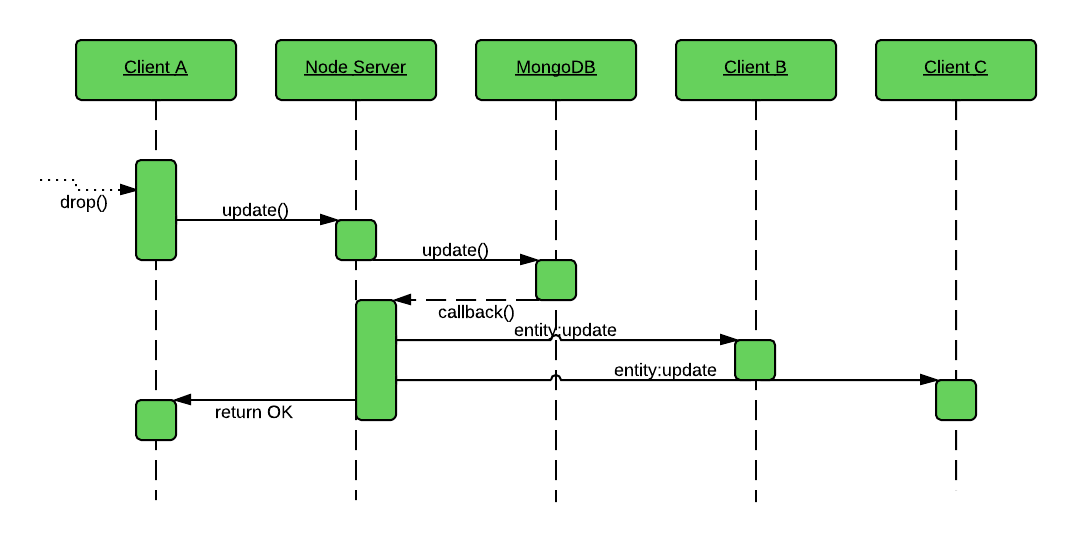
\includegraphics[width=15cm,keepaspectratio]{figures/collaboration-seq.png}
\caption{Entitás módosítás feldolgozása}
\label{fig:entityupdate}
\end{figure}

\begin{lstlisting}[caption=Entitás módosítás feldolgozása szerveroldalon, label=entupdate]
update = function(req, res) {
    var oid = mongo.BSONPure.ObjectID(req.params.id)
    delete req.body._id
    entities.update({_id: oid}, req.body, {upsert:true}, function(err, data){
      if (err) throw err;
      var updated = req.body;
      updated._id = req.params.id;
      socketadapter.broadcast(req.body.document,"entity:update",{msg: "updated", obj: updated});
      res.json(data);
    })
  }
\end{lstlisting}

A~\ref{fig:entityupdate} ábrán és a~\ref{entupdate} kódrészletben azt látjuk, hogyan zajlik a módosításokról való értesítés:

\begin{enumerate}
\item A kliensoldal meghívja az entitás módosító API-t,
\item a módosítások belekerülnek az adatbázisba,
\item ha ez sikeresen zajlik, csak akkor értesítjük a klienseket websocket broadcast segítségével, 
\item válaszolunk az eredeti HTTP kérésnek, a kódrészletben látszik, hogy semmilyen különleges szerializáció vagy transzformáció nincs az adatbázisból kiszedett adatokon.
\end{enumerate}


\subsection{Diagramok másolása}

A JSFiddle egyik funkcionalitása a projekt ``fork''-olása, ami azt jelenti, hogy lemásolódik és új egyedi linken érhető el. Ebben az alkalmazásban is implementálni akartam a diagram másolását és kiderült, hogy egy nagyon érdekes próbléma szerver oldalon a jelenlegi adatbázis séma mellett. Az implementáció lépései a következők:

\begin{enumerate}
\item A kliensoldalon meghívjuk a fork API-t, példáúl 

\url{/api/fork/5242aa48ddda9b0000000001/} címen,
\item a fork API lekérdezi az adatbázisból a diagramot,
\item megváltoztatja a cím  attribútumát és kitörli az azonosítóját, így a következő lépésben ha ezt beszúrja akkor új rekord jön létre, ami a régi másolata,
\item adatbázisból lekérdezi a régi diagram entitásait, 
\item a régi entitások azonosítóját bemásolja az \lstinline{oldid} attribútumba majd kitörli az azonosítót és beállítja az új diagram azonosítót. A végén visszaírja az adatbázisba, így ismét új rekordok jönnek létre,
\item most hogy az új diagram és entitások megvannak és azonosítójuk is van, az új diagram \lstinline{connections} tömbjében a régi entitásokra mutató azonosítókat ki kell cserélni az újakra,
\item még egyszer el kell menteni az új diagramot,
\item vissza kell térni a HTTP kérésre egy válasszal,
\item a kliens betölti az új diagramot.
\end{enumerate}


A végén létrejön az eredeti diagram másolata mindenestül és függetlenül lehet szerkeszteni a két diagramot, továbbfejlesztési lehetőségként elképzelhető egy \lstinline{merge} funkció, ami összefésül két diagramot. 

Ez egy nagyon jó példa arra, amit nehéz megszokni NodeJS-ben, pontosabban az, hogy mivel ez a kód aszinkron, a fenti lépések miatt a kód legmélyebb része már a tizedik indentáció mélységen van és már nem fér ki vízszintesen a kódszerkesztőben. Ilyenkor megoldás az, hogy a callback függvénynek nevet adunk és a fő függvény törzsén kívül deklaráljuk:

\begin{lstlisting}[caption=A \emph{callback pokol} elkerülése]
var updatecallback = function(err, data, res) {
    res.json(data);
}

var update = function(req, res) {
    entities.update({_id: oid}, req.body, {upsert:true}, updatecallback(err, data,res))
}
\end{lstlisting}

Ezt a szituációt callback ``pokolnak'' hívják és van rá megoldás különböző modulokban mint példáúl async.js, aminek segítségével egymásbaágyazott callback hívások helyett függvényláncolást használunk.

%----------------------------------------------------------------------------
\section{A kliens oldali alkalmazás}
%----------------------------------------------------------------------------



Az AngularJS alkalmazásomnak a fő építőelemei a szolgáltatások, direktívák és kontrollerek. A kontrollerek a DOM egy részéért felelnek összekapcsolva a modellt és a view-t; a direktívák a HTML kiterjesztését valósítják meg új elemekkel, amik újrafelhasználható UI komponenseket hoznak létre; a szolgáltatások ugyancsak újrafelhasználható függőségek, amiket tetszőleges más komponensbe lehet injektálni.

A kliens oldali alkalmazás külső függőségei: 
\begin{enumerate}
\item az AngularJS könyvtár, 
\item az underscoreJS könyvtár ami funkcionális programozási elemekkel bővíti a nyelvet,
\item egy md5 hash-t számoló függvény,
\item Jquery UI a DOM elemek mozgatása miatt,
\item PlumbJS ami DOM elemeket köt össze nyilakkal.
\end{enumerate}

Az első próbálkozásaimban nyilakat a HTML SVG path segítségével próbáltam megvalósítani úgy, hogy adatkötés segítségével frissült a nyíl pozíciója egy elhúzott DOM elemhez képest. Sok funkcionalitást kellett volna implementálnom, így kerestem alternatívákat. A PlumbJS egy élhúzó modul aminek segítségével DOM elemeket meg lehet jelölni mint él kiindulópont vagy végpont és ezt a kettőt összeköti egy SVG alapú vektoros nyíllal. Gondoskodik az új él behúzásáért, nyilvántartja a létrehozott éleket, DOM elem körül egy kerületet kell defineálni és ahhoz kapcsolja az élek végpontjait. Továbbá tud nyilat húzni és cimkét tenni a vonalra; azt a következtetést vontam le, hogy mindent tud, amire szükségem van.  

\subsubsection{Jade markup}

A Jade egy olyan markup nyelv ami HTML-t helyettesít, az a fő különbség, hogy a fa nem XML alapú, hanem a gyerekek indentációval különülnek el a szülőtől, ez amúgy is általánosságban szokás, viszont így nincs rá szükség, hogy be is zárjunk HTML elemeket. Az eredmény karakterszámon spórol és olvashatóbb markupot eredményez. A Jade template a Node alkalmazásban fordul le HTML tartalommá. A Jade valóban template rendszer is, tartalmaz példáúl elégazásokat, de én csak markupként használtam, a logika az az Angular kontrollerekre van bízva.

Template öröklés úgy működik, hogy az \lstinline{extends} paranccsal megjelöljük, hogy melyik template a szülő template. A szülőben \lstinline{block} elemeket hozhatunk létre és az ezekben levő DOM rész felülírható a gyerek template-ben. 

Egy hasznos funkció benne a kikommentezés, ami úgy használandó mint a Javascript egy soros komment, viszont a szülő kikommentezése a gyerekek kikommentezését is maga után vonja, így se két helyen nem kell kommentezési parancsot tenni a markupba (a HTML esetében nyitó és záró komment tag kellett) se kiválasztani nem kell a kommentezendő DOM részt.

\begin{lstlisting}[caption=Példa Jade markup]
table
  tr
    td(style='width: '+(100/2)+'%').
      Twitter
    td Facebook
\end{lstlisting}

\begin{lstlisting}[caption=Az ekvivalens HTML]
<table>
  <tr>
    <td style="width: 50%">Twitter</td>
    <td>Facebook</td>
  </tr>
</table>
\end{lstlisting}

%----------------------------------------------------------------------------
\subsection{Direktívák}
%----------------------------------------------------------------------------

\subsubsection{ntDraggable}

Az ntDraggable direktíva a mozgatható diagram dobozokat valósítja és a 

\begin{lstlisting}
<div ng-repeat="entity in shared_document.entities" nt-draggable="nt-draggable" class="drag"></div>
\end{lstlisting}


kód szúrja be őket a DOM-ba. Az adatkötésnek köszönhetően, ha az entities tömb bővül, vagy ritkul, vagy egy eleme megváltozik, akkor ez a DOM-ban is érvényesül. Ez a direktíva egy HTML template-t is meghatároz a mozgatható entitásnak, gyakorlatilag olyan mintha az eredeti DOM-ban lenne ez a HTML, de, ha új helyre szeretnénk másolni a funkcionalitást nem kell lemásolni. A template a következőket tartalmazza:

\begin{enumerate}
\item Egy gyerek div elem ami a \lstinline|{{entity.title}}| kötésen keresztül a doboz nevét írja ki,
\item A model megváltozása esetében a pozíciót is tudom frissíteni CSS attribútumra való kötéssel: \lstinline| style='top:{{entity.position.top}}px;left:{{entity.position.left}}px'|
\item Egy entitás kiválasztása esetében egy CSS osztályt kell hozzáadni a szülőhöz, jelezve, hogy ki van választva. Az AngularJS szolgáltat erre egy \lstinline{ng-class} direktívát ami feltételes CSS osztály beállítást valósít meg. 
\item \lstinline|id={{entity._id}}| Az entitás adabázis azonosítója egy az egyben a DOM id lesz -- egy nagyon kézenfekvő megoldás.
\item A többi felhasználó kijelölését egy kis doboz jelöli, ami a felhasználóhoz rendelt színnel lesz kiszínezve.
\end{enumerate}

\begin{figure}[!ht]
\centering
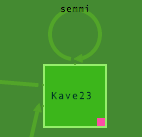
\includegraphics[keepaspectratio]{figures/entitydirective.png}
\caption{ntDraggable mozgatható entitás más felhasználó által megjelölve}
\label{fig:entitydir}
\end{figure}

Az ntDraggable direktíva egy \lstinline{link} függvényt is meghatároz, ennek a törzse pont az a hely ahova a DOM manipuláció és eseménykezelő logikát akarjuk tenni -- pontosabban itt az egérrel való tologatást állítom be. Itt látszik, hogy ez a DOM manipuláció függetlenítve van a prezentációs rétegtől és az alkalmazás többi részétől, ami tesztelhetőség és újrafelhasználás szempontjából értelmes. 

Ahhoz, hogy a div mozgatása a jsPlumb élek mozgatását vonja maga után nem \lstinline{jQuery.draggable}-t kell használni, hanem \lstinline{jsPlumb.draggable}-t, ami kiterjeszti az előbbit. A DOM irányából a kötés a modelhez csak a \lstinline{stop} draggable eseményre történik, mert nem akarunk minden egérmozgatásról értesíteni a többi felhasználót, az nem csak hogy pazarló lenne, hanem zavaró is, így csak akkor terjed a módosítás, ha új helyre engedjük el a dobozt.

Az élhúzás egyszerűség kedvéért ugyancsak egér kattintás és húzogatással történik, de nem a dobozt húzzuk, hanem a nevét, ekkor a jsPlumb gondoskodik az új ideiglenes lógó él kirajzolásáról. Ehhez jsPlumb \lstinline{makeSource} és \lstinline{makeTarget} parancsokat kell hívni, ezek beállítják a cím dobozokat mint cél és forrás a jsPlumb élekhez.

Megjegyzendő, hogy direktívák használata miatt a kontroller és a DOM template nincs csatolva a jsPlumb modulhoz, tehát, ha lecserélnénk a jsPlumb megoldást egy sajátra, ez remélhetőleg csak a direktíva módosítását vonja maga után.

\subsubsection{saveSelected}

A szerkesztő kontrollere nyilvántartja a kiválasztott entitást a gráfban, egy korábbi verzióban kettőt is lehetett kiválasztani, majd ezeket össze lehetett gombnyomással kapcsolni éllel, de ez helyettesítve lett a fennebb említett felhasználói szempontból egyszerűbb megoldással. 

Kijelöléskor az entitás attribútumai megjelennek a részlet nézeten és itt lehet módosítani példáúl a címét. Az adatkötés elintézi, hogy az input doboz tartalma megegyezzen mindkét irányba a modellel, de ettől még nem fognak propagálódni a módosítások a szerverre. 

\begin{figure}[!ht]
\centering
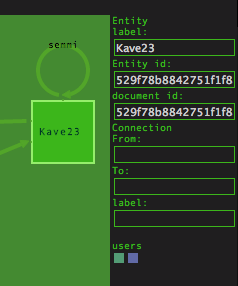
\includegraphics[width=6cm,keepaspectratio]{figures/attributes.png}
\caption{Entitás részletei és többi kapcsolódott felhasználó}
\label{fig:entityattr}
\end{figure}

Ez a direktíva azt csinálja meg, hogy amilyen input elemhez csatoljuk, annak a fókusz elvesztése a kijelölt elem szerverre való mentését váltja ki. A \lstinline{saveSelectedCon} direktíva hasonlóan élek szerverre mentését váltja ki.


\subsubsection{ntDelete}

Az ntDelete direktíva a billentyű funkciókért felelős, amiből kettő van: entitás létrehozás (E gomb) és törlés (backspace gomb). A triviális megoldás az, hogy a document elemre egy \lstinline{keydown} eseménykezelőt állítunk be. Ez sajnos nem elég, mert, ha éppen szöveget szerkesztünk az oldalon, akkor arra is reagálni fog. A direktíva eseménykezelője megkülönbözteti, hogy az eseményt fogadó elem input vagy textarea elem-e és ha igen, akkor az alapértelmezett működés következik be, egyébként meg a backspace hatására az éppen kijelölt entitást vagy élt kitörli.

Fontos megjegyezni, hogy az olyan callback, ami nem AngularJS része, példáúl egy jQuery eseménykezelő, nem fogja a DOM frissítését kiváltani, tehát ha backspace gombnál kitörlünk egy entitást a model listából, ez a DOM-ban nem fog érvényesülni, ilyenkor \lstinline{$scope.$apply();} parancsot kell hívni. 

%----------------------------------------------------------------------------
\subsection{Szolgáltatások}
%----------------------------------------------------------------------------

\subsubsection{SocketService}

A websocket kezelés egy tökéletes példa saját AngularJS szolgáltatásra, ezt akár több kontroller, direktíva vagy szolgáltatásba szeretnénk injektálni és fontos lenne a könnyű hozzáférés és a scope frissítés \lstinline{$scope.$apply();} segítségével. Pontosan ez történik, a SocketService kapcsolódik a szerveroldali Socket.IO szerverhez, majd apply blokkban futtatja a socket üzenet küldés (emit) és fogadás (on) callback metódusokat.

Így kontrollerből átlátszóan használom ezt az adapter és ez a következőképpen néz ki kontrolleren belül:

\begin{lstlisting}[caption=Függőséginjektálás kontrollerbe]
 function EditorCtrl($scope,socket, ...) {
    socket.on('entity:create', function (data) {
      var entities = $scope.shared_document.entities;
      entities.push(data.obj);
    });
 }
\end{lstlisting}

\subsubsection{API szolgáltatások}

AngularJS az alacsonyszintű \$http szolgáltatást kínálja egyszerű AJAX hívásokra, de, ha egy API-val dolgozunk, akkor a \$resource egy olyan absztraktabb szolgáltatás ami REST-szerű API-khoz való kapcsolódást valósít meg. Ekkor saját szolgáltatást kell defineálni egy endpoint megadásával és a műveletek meghatározásával:


\begin{lstlisting}[caption=Szerveroldali erőforrás csomagolása AngularJS-vel]
  app.factory('DocumentService', ['$resource', function($resource){
  return $resource('/api/docs/:id', {id:'@_id'}, 
    { update: {method:'PUT' } , 
      query: {method:'GET', isArray: true}});
    }]);
\end{lstlisting}


Látható, hogy a saját DocumentService API-nek a \$resource a függősége, az \url{/api/docs/:id} URL-hez kapcsolódik és kibővítettem két metódussal ami az update és a query metódus. 

Új entitás létrehozásakor kevés kódot kell futtatni:
\begin{lstlisting}[caption=Új entitás létrehozása]
 $scope.addEntity = function() {
    EntityService.save({ 
      position: {"left":300, top:300 },
      title:"*", 
      document: $scope.shared_document._id}, 
      function(res){}
    )
  }
\end{lstlisting}

\subsubsection{JSPlumbService}


A laza csatolás szem előtt tartása miatt a jsPlumb hívások is egy szolgáltatásban vannak és nincsenek a kontroller vagy view-hoz szorosan csatolva. 

Ez a szolgáltatás beállítja az alapértelmezett jsPlumb paramétereket:

\begin{enumerate}
\item az élek görbülésének mértéke és stílusa,
\item az élek színe, vastagsága,
\item a végpontok stílusa,
\item egy overlay beállítása, ami nyilat valósít meg,
\item  rögzítési pont -- ez esetben folytonos -- ami azt jelenti, hogy nem diszkrét számú pontra illeszkedhet, hanem a doboz kerülete mentén egy közelebbi ponthoz fog kapcsolódni a másik doboz helyzetéhez képest.
\end{enumerate}

Két metódust szolgáltat: új élek létrehozása és egy új diagram betöltésekor  vagy váltáskor az élek felrajzolása egy éllista alapján.
Nincsen adatkötés az élek és az AngularJS modellek között, ezért itt kell ezt megvalósítani.

\subsection{Függőségek vizualizálása}

\begin{figure}[!ht]
\centering
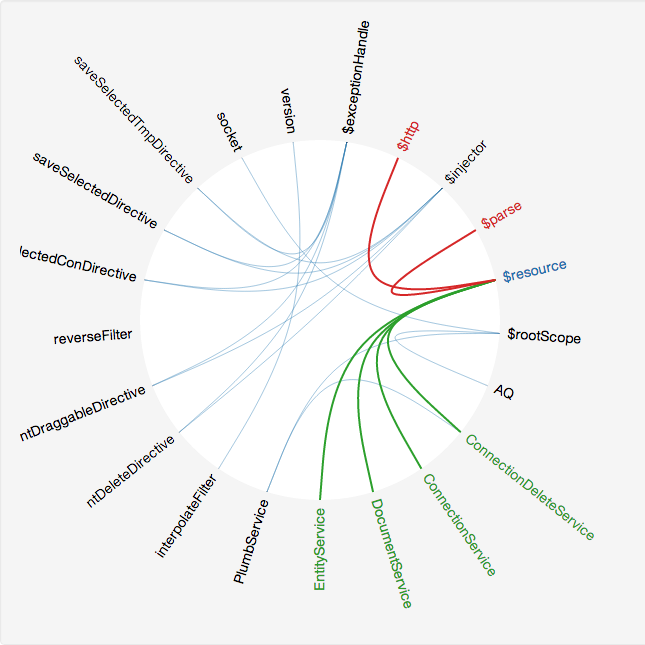
\includegraphics[width=15cm,keepaspectratio]{figures/dependencies.png}
\caption{Függőségek vizualizálása AngularJS chrome toolbar-ban}
\label{fig:angulardependencies}
\end{figure}



A Batarang nevű kiegészítés\footnote{\url{https://github.com/angular/angularjs-batarang/blob/master/README.md}} a Google Chrome böngészőhöz egy AngularJS debuggoló eszköz, a ~\ref{fig:angulardependencies} ábrán látszik a függőségek vizualizálása, ami az egyik eszköz a Batarang-ban. A kör mentén fel vannak sorakoztatva a beépített -- általában \$-vel kezdődő nevűek -- és a fejlesztő által implementált komponensek: szolgáltatások, direktívák, filterek. A függőségi gráfban egy komponenst kiválasztva zöld színű élek mutatnak az őt felhasználó komponensekre, a pirosak meg azokra mutat akiket ő használ fel.




\subsection{A szerkesztő kontroller}

\begin{itemize}
\item A kontroller betöltésekor lekéri a DocumentService-től az összes diagramot és majd az elsőt betölti,
\item defineál egy inicializáló metódust ami a diagram betöltését valósítja meg. Ekkor bizonyos változók újra az eredeti értéküket kapják meg, majd frissülnek az API-ból a diagram adatai, az entitásokat lekéri és inicializálja az éleket. A végén Websocket üzenetet küld arról, hogy az új diagramra váltott és a szerveroldalon egy másik socket szobába kerül;
\item lehetővé teszi az új diagram létrehozását,
\item lehetővé teszi az entitások kiválasztását, ami kitörli az esetleges jelzést értesíti a többi felhasználót,
\item diagram manipuláció Websocket üzenetekre deklarál kezelőket, ezek az üzenetek a következők:
\begin{itemize}
\item entity:create
\item entity:update

A végén meg kell hívni az összes él újrarajzolását. Ehhez egy 0 idejű setTimeout egy trükk, hogy a keretrendszer kód lefutása után futtassunk valamit: \lstinline|setTimeout(function(){jsPlumb.repaintEverything()},0)|

\item entity:delete

Ekkor törölni kell az éleket a jsPlumb segítségével, hogy ne legyenek lógó élek.

\item connection:create
\item connection:delete

\end{itemize}

\item a \lstinline{chat} üzenet kezelőjében nyilvántartásba veszi a csatlakozott felhasználókat,
\item a \lstinline{mark} üzenet kezelőjében frissíti az entitás megjelöléseket,
\item a \lstinline{sync} üzenet kezelőjében összeegyezteti a saját diagram hash lenyomatait a többi felhasználóéval,
\item entitások és élek manipulálására szolgáló segédfüggvények,
\item a diagram változásaira figyelő függvényt kapcsol, ez rendszeresen lenyomatot számol a gráfból.

\end{itemize}



\label{subsec:hashref}
%----------------------------------------------------------------------------
\subsection{Diagram hash}
%----------------------------------------------------------------------------

Ahhoz, hogy össze lehessen hasonlítani két különboző kliens által látott diagramot kézenfekvőnek tartottam egy hash értéket számolni a diagram alapján. A hash értéke úgy számolódik, hogy a diagram entitásait azonosító szerint sorrendezem és egy tömbbe pakolom, majd a tömb szerializált formájából egy MD5 hasht számolok. Mivel sorrendezve vannak az entitások várhatóan két egyforma diagramnak ugyanaz lesz a hash értéke.

A hash számolása nem explicit módon van meghívva, hanem egy AngularJS eszköz segítségével, a \lstinline{watch} paranccsal, ami a modell egy részének a változásait figyeli és a beállított callback metódust meghívja, ha változik a modell.

\begin{lstlisting}[caption=Modell módosításaira meghívódó callback]
  $scope.$watch('shared_document.entities', function (newVal) {
      ...
  }, true);
\end{lstlisting}

A szerkesztő kontroller kontextusában egy FIFO tömb van ami hash értékeket tárol.

Az \lstinline{inactive} változó értéke azt jelzi, hogy éppen szerkesztünk-e és ez ugyancsak egy \lstinline{watch} segítségével hamisra állítódik, ha elég régóta nem változtatott senki semmit a diagramon. Amikor ez az érték hamisra állítódik egy broadcast üzenetet küld az alkalmazás a többi felhasználónak, amiben a hash értékek tömbjét küldi el. A fogadó oldalon erre a \lstinline{sync} socket üzenetre a kliens összehasonlítja a saját hash tömbjét a kapott tömbbel és ha eltérés van, akkor jelez az alkalmazás, hogy nem egyezik meg a két diagram.

Ez a késleltetés megoldja azt a nehézséget, hogy két kliens normális körülmények között nem feltétlenül látja mindig ugyanazt a diagramot, de ha senki nem változtatott egy ideje, akkor viszont ugyanazt kellene, hogy lássák, tehát akkor kell ellenőrizni.


%----------------------------------------------------------------------------
\section{Pehelysúlyú zárolás}
%----------------------------------------------------------------------------

Ahelyett, hogy megakadályozzam, hogy a többi résztvevő felhasználó, ne változtathassák bizonyos részeit a diagramnak, csak egy jelzési mechanizmust implementáltam, amivel láthatóvá válik, ha valaki kijelölt egy entitást. Ehhez először szükség van a szoba résztvevők nyilvántartására, hiszen a kollaborációhoz nem volt kötelező tudni, hogy ki nézi még a diagramot.

Szerencsére szerveroldalon a Socket.IO könnyen elérhetővé teszi ezt az információt: \lstinline{io.sockets.clients(szoba);} egy socket objektumokból álló tömböt ad vissza. A \lstinline{connection} és a \lstinline{disconnect} események hatására értesül a szerveroldal arról, hogy valaki kapcsolódott, vagy elhagyta a szobát.

\begin{figure}[!ht]
\centering
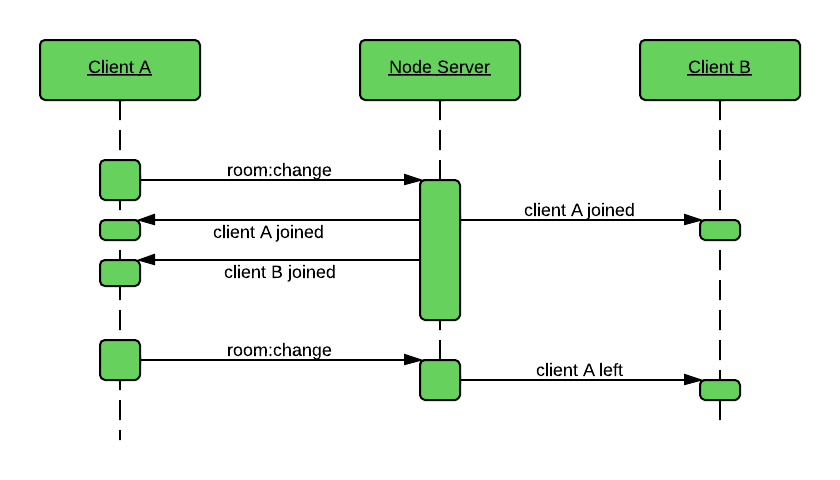
\includegraphics[width=15cm,keepaspectratio]{figures/join-seq.png}
\caption{Felhasználó belép a szobába}
\label{fig:joinseq}
\end{figure}

Az ábrán látszik, hogy szoba váltáskor a szerveroldal minden résztvevőjét a szobának (az új résztvevőt beleértve) értesít arról, hogy belépett, és az új résztvevőnek a létező socketek listáját is elküldi. Kilépéskor vagy diagram váltáskor is értesíti a klienseket. Így a kliensek nyilvántartást tudnak tartani a kapcsolódott többi kliensről. A \lstinline{client joined} és a \lstinline{client left} üzenetek esetében -- mivel az alkalmazás nem használ felhasználói fiókokat -- egy socket példány azonosítót is küld a kliensnek.

A socket azonosítókhoz színeket lehet nagyon egyszerűen rendelni úgy, hogy md5 hash-t számoltatok az azonosítóból és így egy hexadecimális értéket kapok. Ennek elég 6 betűjét venni és már megvan egy -- nagy valószínűséggel -- egyedi szín, legalábbis egy megnyitott diagramon belül.

Ez a jelölés a ~\ref{fig:entitydir} ábrán is látszik. 

A jelöléseket egy kulcs-érték objektum tartalmazza, a kulcs az entitás azonosító, az érték az felhasználó színazonosítója. Ez a reláció irány azért hasznos, mert az entitás direktíva közvetlenül tud erre a színre hivatkozni:

\begin{lstlisting}
 <div class='entity_mark' style='background-color:#{{marks[entity._id]}};'>
 </div>
\end{lstlisting} 

tehát, ha van az objektumban egy konkrét entitás azonosító mint kulcs, akkor megjelenik egy olyan színű doboz, ha nem, akkor nem látszik semmi. 

Viszont, amikor egy másik kliens jelöléséről értesülünk, akkor egy entitás azonosítót és egy kliens azonosítót kapunk, ekkor nagyon kézenfekvő lenne a fordított irányú kulcs-érték objektum, vagyis kliens azonosítókhoz rendelt entitás azonosító. Ha ez meglenne, akkor egy műveletben kicserélnénk a régi jelölését az újra. Szerencsére az underscoreJS eszközkészletében találunk dictionary megfordítót:

\begin{lstlisting}
    socket.on('mark', function (data) {
        var inverted = _.invert($scope.marks)
        // user->id
        $scope.marks[inverted[data.user]] = null;
        $scope.marks[data.id] = data.user;
    });
\end{lstlisting}

Itt látszik, hogy ez a broadcast is szokásosan Socket.IO segítségével történik.


\section{Vizuális programozási nyelvek és kódgenerálás}

\begin{figure}[!ht]
\centering
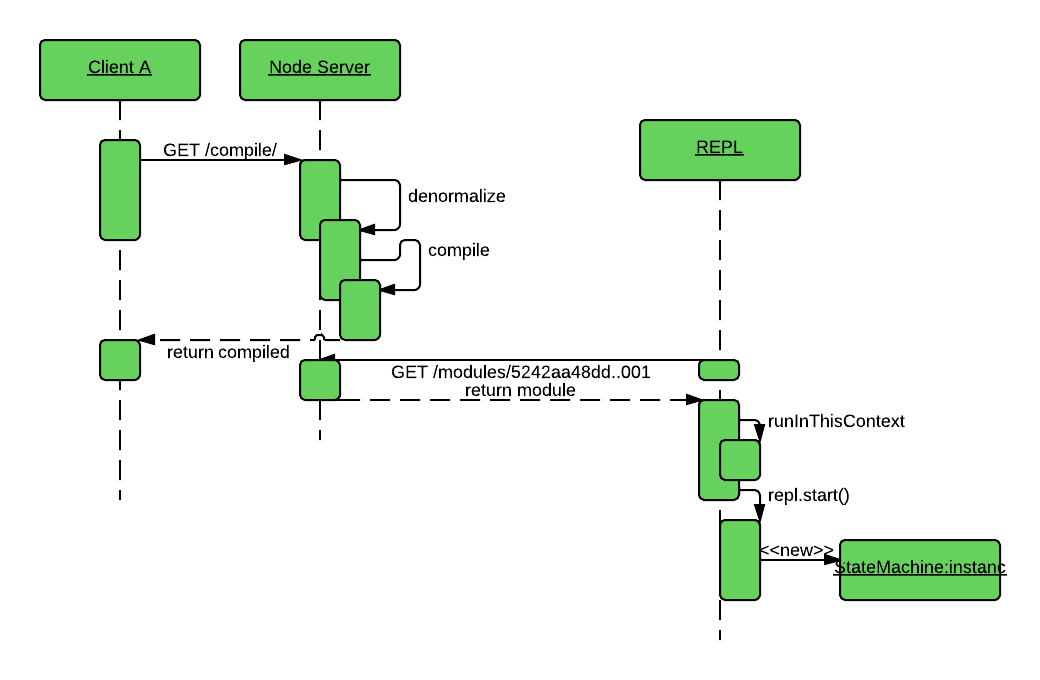
\includegraphics[width=15cm,keepaspectratio]{figures/compile-seq.png}
\caption{Kódgenerálás}
\label{fig:compileseq}
\end{figure}

A kollaboratív gráfszerkesztésen túl az alkalmazás egyszerű vizuális programozási nyelvek létrehozására alkalmas.
A vizuális programozás menete a következő egy minta nyelv példányán amiben állapotgépeket lehet programozni:
\begin{enumerate}
\item A kliensoldalon a felhasználó elkészíti a gráftranszformációs template kódot,
\item A felhasználó elkészíti egy vizuális implementációját a nyelvnek, vagyis egy konkrét állapot gépet vizuálisan,
\item A fordítás gomb megnyomása után a szerveralkalmazás denormalizálja a gráfot, azaz létrehoz egy olyan struktúrát, ami a diagramot reprezentálja redundánsan. Ez a struktúra a bemenő adata a gráftranszformáló template-nek,
\item A szerveralkalmazás a template alapján egy konkrét állapotátmenetekkel rendelkező állapotgép Javascript kódját hozza létre,
\item Ezt a kódot elmenti az adatbázisba és választ küld a kliensalkalmazásnak, ekkor kétféleképpen lehet felhasználni a kódot:
\begin{enumerate}
    \item A felhasználó böngészőjének Javascript parancssorában (példáúl Chrome Developer Console) értelmezi a kódot \lstinline{eval} segítségével és példányosítja az állapotgépet. 
    \item Node.JS parancssorból a mintrepl segédalkalmazással betölti a kódot, majd példányosítja az állapotgépet.
\end{enumerate}
\end{enumerate}


\subsubsection{Denormalizálás}

Az eredeti ``séma'' csúcsok listáját és élek listáját jelenti, viszont ez az adatformátum nem hasznos relációk kezelésére. Ezért reláció helyett redundancia bevezetésével oldom meg: egy diagram ilyen reprezentációjában egy él többször is jelenik meg. Ez leegyszerűsítve így néz ki:

\begin{lstlisting}
    {   edges: [
            {from: a, to: b},
            {from: a, to: c}],
        points: [
            {name: a, outgoing: [{from: a, to: b},{from: a, to: c}], incoming: []},
            {name: b, outgoing: [], incoming: [{from: a, to: b}]},
            {name: c, outgoing: [], incoming: [{from: a, to: c}]},
        ]
    }
\end{lstlisting}

Így ezen a struktúrán kevesebb kóddal írható egy olyan transzformáció ami valamilyen logikát valósít meg abból kiindulva, hogy milyen állapotból milyen élek mennek ki és be. Ez struktúra ami ilyenkor létrejön csak átmenetileg van felhasználva amíg kódot generál a szerveroldal, utána nem lesz használva semmire, így nem kella redundancia által okozott szokásos próblémákkal küzdeni. Ebben a formában tárolni mindig a gráfot nem hatékony, mert minden diagram manipulációs művelet több mint egy adatbázis lekérdezést jelentene és ha el szeretném kerülni a redundancia anomáliákat 
akkor megnövekedne fölöslegesen a komplexitás (tranzakciókra lenne szükség, vagy zárolásra és ezeket nem biztosítja a MongoDB). Ez a denormalizálás viszont csak két for ciklusból áll és ritkán fut le. 

\subsubsection{Gráftranszformáció template}

A gráftranszformáció template egy Underscore template. Underscore.JS egy Javascript könyvtár ami funkcionális programozás eszközökkel bővíti e nyelvet, anélkül, hogy kiterjesztené a beépített típusokat. \cite{underscorejs.org}
Ezen belül a template rendszer lehetővé teszi egy template fájlt lefordítását adott kontextus alapján. A template-ben \lstinline{<\%= \%>} segítségével változó behelyettesítés történik, \lstinline{<\% \%>} segítségével Javascript kódot lehet értelmeztetni. 

\begin{lstlisting}
var compiled = _.template("hello: <%= name %>");
compiled({name: 'moe'});
=> "hello: moe"
\end{lstlisting}

Az alkalmazásban így néz ki felhasználói szemszögből:

\begin{figure}[!ht]
\centering
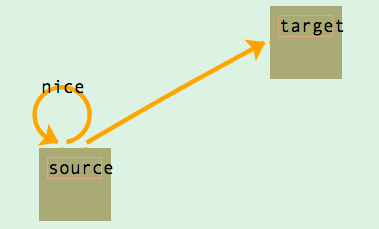
\includegraphics[width=5cm,keepaspectratio]{figures/simple-graph.png}
\caption{Egy példa diagram}
\label{fig:compileseq}
\end{figure}

\begin{lstlisting}[caption=A template]
Elements: 
<% 
    doc.entities.forEach(function(el){
%>
    <%= el.title %>
<%
    })
%>
\end{lstlisting}

És a kimenet: 
\begin{lstlisting}[language=HTML]
Elements: 

source
target
\end{lstlisting}

Természetesen nem csak Javascript kódot lehet generáltatni az alkalmazásban, hiszen a template behelyettesítés eredménye egyszerű szöveg. 






%---------------------------------------------------
\subsubsection{A generált kód felhasználása}
%---------------------------------------------------

A generált kód elmentődik az adatbázisba a diagram egyik attribútumába, és ehhez az adathoz egy API végponton keresztül lehet hozzáférni és felhasználni meg akár a triviális HTML script elem segítségével:

\begin{lstlisting}[language=HTML]
 <script type="text/javascript" src="http://localhost:3000/api/compile/modules/5242aa48ddda9b0000000001/"></script>
\end{lstlisting}

Parancssorból is fel lehet használni \lstinline{node mintrepl <id>} segítségével, a mintrepl egy javascript szkript, ami a fent említett API-n keresztül letölti és értelmezi a fájlt, majd futtatja a letöltött kódot és egy REPL\footnote{Read-Eval-Print-Loop} interaktív node shell-t futtat. 

\begin{lstlisting}
 $ node mintrepl 5242aa48ddda9b0000000001
 mint 5242aa48ddda9b0000000001> tanulo = new sm()
 mint 5242aa48ddda9b0000000001> tanulo.consumeEvent("kávé")
 mint 5242aa48ddda9b0000000001> tanulo.currentState
 ébren
 \end{lstlisting}

 Hasonló módon egy másik node szerver szerveroldali kódjába is be lehet illeszteni. 
 










